\documentclass[12pt]{report}  % Defines the document type

\usepackage[a4paper, margin=1in]{geometry} % Page layout including papter size and margins
\usepackage{newtxtext,newtxmath}  % For Times-like font with text (newtxtext) and math (newtxmath) support
\usepackage[utf8]{inputenc} % Character encoding in this .tex file
\usepackage[T1]{fontenc} % Text rendering and font encoding
\usepackage{amsmath} % Better math

\usepackage{enumitem}  % For customized itemize environments
\usepackage{graphicx}    % Allows inserting images
\usepackage{url}

\usepackage{caption}
\usepackage{forest}
\usepackage{float}
\usepackage{tikz}
\usepackage{subcaption}

\usepackage{booktabs}
\usepackage{array}
\usepackage{pgfplots}

\pgfplotsset{compat=1.18}

\usetikzlibrary{arrows.meta, positioning}

\begin{document}         % Start of the document content

% Centering all content vertically and horizontally
\begin{center}

% Adding space at the top
%\vspace*{1cm}

% Adding the institution header
{\Large \textbf{People’s Democratic Republic of Algeria}} \\
\vspace{0.3cm}
{\large Ministry of Higher Education and Scientific Research} \\
\vspace{0.3cm}
{\large University M'hamed Bougara - Boumerdes} \\
\vspace{1cm}
% Including the logo
% Adjust the width as needed; assumes the logo file is named 'logo.png' and is in the same directory
\includegraphics[width=0.5\textwidth]{cropped-logo1.png}

% Adding vertical space after the logo
\vspace{1cm}


% Faculty and department
{\large \textbf{Faculty of Sciences}} \\
\vspace{0.3cm}
{\large Department of Computer Science} \\
\vspace{1cm}


% Program details
\begin{flushleft}
\renewcommand{\arraystretch}{1.5}
\begin{tabular}{ll}
\textbf{Field} & : Mathematics and Computer Science \\
\textbf{Program} & : Computer Science \\
\textbf{Specialization Accreditation Decree No.} & : Decree No. 872 of 26/07/2016 \\
\end{tabular}
\end{flushleft}
\vspace{1cm}

% Degree information
{\large \textbf{End-of-Studies Thesis for the Obtainment of the}} \\
{\large \textbf{Academic Bachelor’s Degree}} \\
\vspace{1cm}

% Theme section
{\large \textbf{Theme}} \\
{\large Reinforcement Learning} \\
\vspace{1cm}

% Student names
{\large \textbf{Presented by}:} \\
Abdellaoui Mohammed\\
Ait-Ameur Mohamed Ilyas \\
Gaceb Hicham\\
\vspace{1cm}

% Defense details
{\large \textbf{Defended on} 24/05/2025 \textbf{Before the Jury Composed of}:} \\

    \begin{center}
\renewcommand{\arraystretch}{0.5}
\large Djerbi Rachid: \textbf{Examiner} \\
\large Berrichi Ali: \textbf{Supervisor} \\
\vspace{1cm}
    \end{center}


\end{center}


\tableofcontents

\section*{Chapter 1: Introduction to Artificial Intelligence}
\addcontentsline{toc}{section}{Chapter 1: Introduction to Artificial Intelligence}
\begin{itemize}
    \item[1.1] Origins \dotfill 2
    \item[1.2] What is Intelligence? \dotfill 3
    \begin{itemize}
        \item[1.2.1] Human Behavior \dotfill 3
        \item[1.2.2] Rational Reasoning \dotfill 4
        \item[1.2.3] Rational Behavior \dotfill 5
    \end{itemize}
    \item[1.3] Machine Learning \dotfill 8
    \begin{itemize}
        \item[1.3.1] Types of Learning \dotfill 8
    \end{itemize}
    \item[1.4] State of the Art in Reinforcement Learning \dotfill 10
    \begin{itemize}
        \item[1.4.1] Recent Advancements \dotfill 10
        \item[1.4.2] Motivations for Studying Reinforcement Learning \dotfill 11
        \item[1.4.3] Challenges and Future Directions \dotfill 11
    \end{itemize}
\end{itemize}

\section*{Chapter 2: Introduction to Reinforcement Learning}
\addcontentsline{toc}{section}{Chapter 2: Introduction to Reinforcement Learning}
\begin{itemize}
    \item[2.1] Core Concepts \dotfill 12
    \item[2.2] The Maze Example \dotfill 14
    \begin{itemize}
        \item[2.2.1] Policy Optimization \dotfill 15
        \item[2.2.2] Code Implementation \dotfill 19
    \end{itemize}
    \item[2.3] Temporal Difference \dotfill 20
    \begin{itemize}
        \item[2.3.1] TD Learning Methods \dotfill 21
        \item[2.3.2] Implementation \dotfill 21
    \end{itemize}
\end{itemize}

\section*{Chapter 3: Advanced Concepts in Reinforcement Learning}
\addcontentsline{toc}{section}{Chapter 3: Advanced Concepts in Reinforcement Learning}
\begin{itemize}
    \item[3.1] Value Functions and Bellman Equations \dotfill 23
    \begin{itemize}
        \item[3.1.1] State-Value and Action-Value Functions \dotfill 23
        \item[3.1.2] Bellman Equations \dotfill 24
        \item[3.1.3] Policy Gradient Methods \dotfill 24
    \end{itemize}
\end{itemize}

\section*{Bibliography}
\addcontentsline{toc}{section}{Bibliography} \dotfill 25

\begin{abstract}
This thesis provides a comprehensive exploration of reinforcement learning (RL), a dynamic subfield of artificial intelligence (AI) focused on enabling agents to learn optimal decision-making through interaction with environments. The study begins with an introduction to AI, tracing its historical and philosophical origins, defining intelligence through human behavior and rational reasoning, and outlining key paradigms, including machine learning. The core of the thesis delves into RL, formalizing its principles through Markov Decision Processes (MDPs) and illustrating them with a maze example. It examines model-free RL methods, such as Monte Carlo and Temporal Difference (TD) learning, comparing their sample efficiency in practical implementations. Advanced concepts, including value functions, Bellman equations, and policy gradient methods, are explored to highlight RL's capability to address complex sequential decision-making tasks. Recent advancements from 2023 to 2025, such as RL from Human Feedback (RLHF) and applications in nuclear fusion, robotics, and healthcare, underscore RL's transformative potential. The thesis also addresses challenges like sample efficiency and safety, emphasizing RL's societal impact and future research directions. Through theoretical insights and practical demonstrations, this work aims to provide a foundational understanding of RL for addressing real-world problems.
\end{abstract}

\chapter{Introduction to Artificial Intelligence}

% Introducing the purpose and scope of the chapter
This chapter provides a comprehensive introduction to the field of Artificial Intelligence (AI), tracing its historical roots and philosophical underpinnings to its modern technical advancements. We begin by exploring the \textbf{origins} of AI, from ancient philosophical inquiries into reasoning to the pivotal contributions of figures like Alan Turing in the 20th century. Next, we address the fundamental question, \textit{What is Intelligence?}, examining contrasting perspectives on human-like behavior versus pure rationality, and how these shape AI's development. The chapter then delves into \textbf{rational reasoning}, introducing logical frameworks such as propositions, truth tables, and proofs that enable machines to reason systematically. We also explore \textbf{rational behavior}, focusing on intelligent agents like expert systems and their parallels with control theory, challenging traditional notions of intelligence. The section on \textbf{machine learning} outlines key paradigms—supervised, unsupervised, semi-supervised, and reinforcement learning—highlighting how algorithms learn from data to solve practical problems. Finally, we review the \textbf{state of the art} in AI, drawing on recent reports to illustrate its rapid progress and societal impact. Together, these sections offer a foundational understanding of AI as a dynamic, interdisciplinary field poised to transform our world.

\section{Origins}

The idea of a thinking machine is an old one. There have been stories of mechanical automatons since the time of Greek mythology and Chinese legends dating back to 1000 BCE. However, people did not seriously attempt to build something of the sort until the mid-1900s, when Alan Turing designed the first theoretical model of a machine that could "think" by processing symbols in 1936. The term "Artificial Intelligence" was coined at the Dartmouth Conference in 1956, marking the formal birth of AI as a field. Meanwhile, other forms of "AI" would appear throughout history. Take for instance Logic-based machines, which are symbolic systems designed to solve logical problems rather than computational ones. Those were conceived as far back as the 17th century, like Blaise Pascal's \textit{Pascaline} in 1642. 

As you may see, what we call today Artificial Intelligence is a fairly recent field. However, the disciplines it builds upon are much older. Philosophers, as far back as 400 BCE, debated the nature of knowledge and its relation to action. Among them was the well-known Aristotle, who would try to grasp the rational part of the mind by developing an informal system of syllogisms for proper reasoning which, in principle, would allow one to generate conclusions mechanically given initial premises. This method would be used to explain how knowledge relates and lead to action by providing a logical connection between goals and the knowledge of the action's outcome. It also constitutes a foundational base for future mathematical logic and even computer engineering. Such a system would, however, posit other philosophical questionings about the relashionship between mind and matter. Descartes (1596–1650) gave the first clear discussion of the distinction between mind and matter. He noted that a purely physical conception of the mind seems to leave little room for free will, thus sparking a philosophical debate that would make it to our modern times.

Other than philosophy, numerous sciences would come together as solutions to the many problems that AI was facing. Mathematics would formalize logic rules to allow computers to draw valid conclusions, which will become the basis that would allow computers to reason logically. It would establish the theory of probability that would allow computers to reason with uncertain informations. Economics answered questions such as decision-making under a constrained environment to achieve long-term goals. Neuroscience would have breakthroughs on how our brains process information, which would inspire AI learning methods. Linguistics studies the relationship between knowledge and thought, which proved to be quite a challenging problem.

In short, AI came at a juncture of science. It encompasses a huge variety of subfields ranging from general learning, reasoning and perception, to the specific, such as playing chess, proving mathematical theorems, writing poetry, driving a car, or diagnosing diseases. This makes AI a field that is relevant to any intellectual task; it is truly a universal field.

To attempt to define it, however, would require us to ask another question: 

\section{What is Intelligence?}

Intelligence has multiple definitions, depending on which school of thought you consult. You can discover where you stand by answering two key questions: \textit{Are you interested in being human, or in pursuing a pure rationality free from human flaws?} And, \textit{Would you say intelligence is a characteristic of the process of thought and reasoning, or simply that of behavior?} 

These distinctions shape AI research priorities, with human-like intelligence driving applications like chatbots, while rational approaches underpin systems like autonomous vehicles.

\subsection{Human Behavior}

If we want to imitate human behavior—meaning that being intelligent is equated with being human, whatever that may mean—and we define intelligence as an attribute of behavior, then we arrive at the \textbf{Turing Test}. Proposed by Alan Turing in 1950, the test was designed as a thought experiment to sidestep the philosophical vagueness of the question, “Can a machine think?” A computer passes the test if a human interrogator, after posing written questions, cannot distinguish whether the responses come from a human or a machine.

Programming a computer to pass such a well-defined test is a substantial challenge. It requires progress in what are now major research areas in AI: natural language processing, knowledge representation, automated reasoning, and more…

These disciplines make up most of the field of AI. Yet AI researchers have devoted relatively little effort to passing the Turing Test, believing it is more important to study the underlying principles of intelligence. The quest for artificial flight succeeded when engineers and inventors stopped imitating birds and instead focused on wind tunnels and aerodynamics. Aeronautical engineering textbooks do not define their field’s goal as building “machines that fly so exactly like pigeons that they can fool even other pigeons.”

In the end, just as we were inspired to fly by watching birds, our fascination with human behavior was simply the spark—born from being captivated by our own existence. But it is certainly not the destination we are striving for.

\subsection{Rational Reasoning}

By choosing not to emulate humans, we pursue a form of perfect rationality—that is, loosely speaking, the ability to do the “right thing” at all times. If we define intelligence as a property of the thought process (rather than mere behavior), then we need a language in which to express that process. That language is mathematical logic.

We call a \textbf{proposition} \textit{p} a claim that can be either true or false (but not both). We can use basic, clearly defined operations to build more complex claims: the formula $p \wedge q$ means \textit{p and q}, and it is true if and only if both \textit{p} and \textit{q} are true. Notice that we just said "if and only if." That sort of phrasing is standard in mathematical writing because its meaning is agreed upon. Linguistically, saying \textit{p when q} is ambiguous. Does it mean that we can assume that \textit{q} is true at the same time as \textit{p}? Could it be that \textit{q} is true without \textit{p} being true? It is these linguistic ambiguities that we are trying to eliminate by using these symbols.

That conditional tool has a symbol: $\textit{p} \rightarrow \textit{q}$ means \textit{if p, then q}. These tools are defined by a \textbf{truth table}. In the case of the conditional statement, the corresponding truth table is:

\vspace{1em} % Adds vertical space before the table

\begin{center}
    \begin{tabular}{|c|c|c|}
        \hline
            $\textit{p}$ & $\textit{q}$ & $\textit{p} \rightarrow \textit{q}$ \\
        \hline
            T & T & T \\
            T & F & F \\
            F & T & T \\
            F & F & T \\
        \hline
    \end{tabular}
\end{center}

We use a truth table because it removes ambiguity and provides a clear, concise definition. You may notice that we can’t fully derive the truth table just from the phrase “if p, then q.” The truth table makes it clear that when \textit{p} is false, the conditional \textit{p} → \textit{q} is treated as true—almost by generous disregard. This convention is convenient because proving a conditional essentially comes down to showing that there is no case where \textit{p} is true and \textit{q} is false. All other scenarios—such as when \textit{q} is true or \textit{p} is false—cause the entire formula to default to true.

In particular, when \textit{p} is false, we still consider the conditional statement to be true. That’s because we are only interested in evaluating the truth value of \textit{q} when \textit{p} is true—not when \textit{p} is false. Again, the core idea is to express, in a single formula, that there is no case where \textit{p} is true and \textit{q} is not. That’s why we treat all other cases as true: they do not violate that one condition.

We can now appreciate the meaning and usefulness of the phrase \textit{“if and only if.”} The statement \textit{"p if q"} is logically equivalent to $q \rightarrow p$, while \textit{"p only if q"} corresponds to $p \rightarrow q$. Therefore, \textit{“p if and only if q.”} translates to the conjunction: 

\[ (p \rightarrow q) \land (q \rightarrow p) \]

This means there is no scenario in which one is true and the other is not. These operators may seem silly at first, but their utility quickly shines when we want to work with \textbf{proofs}. Proofs in mathematics are valid arguments that establish the truth of mathematical statements.

By an \textbf{argument}, we mean a sequence of statements that ends with a conclusion. By \textbf{valid}, we mean that the conclusion—or final statement of the argument—must logically follow from the truth of the preceding statements, or \textbf{premises}. That is, an argument is valid if and only if it is impossible for all the premises to be true while the conclusion is false.

Notice how this aligns precisely with the behavior of the conditional operator we defined earlier. From the definition of a valid argument, we see that an argument in which the premises are $p_1, p_2,\cdots, p_n$ and the conclusion is \textit{q} has the following logical form:

\[ (p_1 \land p_2 \land \cdots \land p_n) \rightarrow q \]

To deduce new statements from existing ones, we use \textbf{rules of inference}—standard argument forms that serve as templates for building valid reasoning steps. Rules of inference are our basic tools for establishing the truth of statements. Like many concepts, it is better understood with an example. Let's consider the following argument involving propositions:

“If you have a current password, then you can log onto the network.”

“You have a current password.”

Therefore,

“You can log onto the network.”

We would like to determine whether this is a valid argument. That is, we would like to determine whether the conclusion “You can log onto the network” must be true when the premises “If you have a current password, then you can log onto the network” and “You have a current password” are both true. Before we discuss the validity of this particular argument, we will look at its form. Use \textit{p} to represent “You have a current password” and \textit{q} to represent “You can log onto the network.” Then, the corresponding \textbf{argument form} is:

\[
\begin{array}{ll}
        p \rightarrow q & \\
        p & \\
    \hline
        \hspace{-0.5cm} \therefore q
\end{array}
\]

where $\therefore$ is the symbol that denotes “therefore." By definition, the logical form of this argument is $(p \rightarrow q) \land p \rightarrow q$. Let's draw it's truth table: 

\[
\begin{array}{|c|c||c|c|c|}
    \hline
        p & q & p \rightarrow q & (p \rightarrow q) \land p & (p \rightarrow q) \land p \rightarrow q \\
    \hline
        T & T & T & T & T \\
        T & F & F & F & T \\
        F & T & T & F & T \\
        F & F & T & F & T \\
    \hline
\end{array}
\]

Notice that the formula is true in \textit{every possible case}, regardless of the truth values of the individual variables. Such a formula is called a \textbf{tautology}. In fact, all rules of inference are based on tautologies—something that becomes evident when you reflect on everything we've built up so far. This particular tautology is known as \textbf{modus ponens} (Latin for \textit{the mode that affirms}).

In principle, this framework would allow the construction of a comprehensive model of rational thought, leading from raw perceptual information to an understanding of how the world works to predictions about the future. What it does not do, is generate intelligent behavior. For that, we need a theory of rational action. Rational thought, by itself, is not enough.

\subsection{Rational Behavior}

An \textbf{agent} is just something that acts (agent comes from the Latin agere, to do). In this paradigm, an agent that behaves rationally is said to be \textit{intelligent}. An example of such an agent would be an \textbf{expert system}. Such systems are considered a form of intelligent agents, particularly in the early symbolic AI era. However, they are rule-based, static, and lack learning capabilities, which distinguishes them from more modern, adaptive intelligent agents. 

An expert system is a computer program designed to simulate the decision-making ability of a human expert. It solves complex problems by reasoning through a set of facts and rules, using a knowledge base and an inference engine to draw logical conclusions. 

\begin{center}
    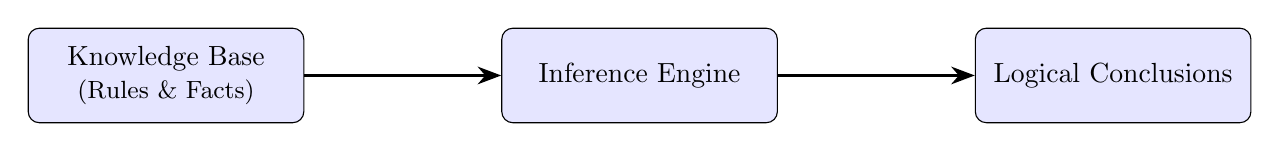
\begin{tikzpicture}[
      box/.style={rectangle, draw, minimum width=3.5cm, minimum height=1.2cm, text centered, rounded corners, fill=blue!10},
      arrow/.style={-{Stealth[length=3mm]}, thick},
      node distance=2cm and 2.5cm
    ]

    \node[box, align=center] (kb) {Knowledge Base \\ \small (Rules \& Facts)};
    \node[box, align=center, right=of kb] (ie) {Inference Engine};
    \node[box, align=center, right=of ie] (out) {Logical Conclusions};

    \draw[arrow] (kb) -- (ie);
    \draw[arrow] (ie) -- (out);

    \end{tikzpicture}
\end{center}

A \textbf{fact} is a statement known to be true. In a symbolic form, we can denote a fact as a propositional symbol, such as $A$, $B$, etc. The sets of facts is thus a set of true propositions. A \textbf{rule} is an implication of the form:

\[ A_1 \land A_2 \land \dots \land A_n \rightarrow B \]

where $A_1, A_2, \dots, A_n$ are premises (conditions), and $B$ is the conclusion. This means that if all the $A_i$ are true (i.e., they are contained in the set of facts), then $B$ can be inferred. The \textbf{inference engine} is the component that applies logical reasoning to derive new facts from existing facts and rules. Two common methods used in expert systems are \textit{forward chaining} and \textit{backward chaining}.

\paragraph{Forward Chaining Algorithm (Data-Driven):}

\begin{verbatim}
    1. Start with a set of known facts.
    2. Repeat:
        a. For each rule:
            - If all premises are known facts and the conclusion is not:
                * Add the conclusion to the set of known facts.
    3. Until no new facts can be inferred.
\end{verbatim}

\paragraph{Example:}

\[ \text{has\_fever} \land \text{has\_cough} \rightarrow \text{possible\_flu} \]

If we know that both \texttt{has\_fever} and \texttt{has\_cough} are facts, forward chaining will deduce \texttt{possible\_flu}.

\paragraph{Backward Chaining Algorithm (Goal-Driven):}

\begin{verbatim}
    1. Start with the goal to prove.
    2. If the goal is already a known fact, return true.
    3. Else, find a rule with the goal as its conclusion.
    4. Try to prove each premise of that rule recursively.
    5. If all premises are proven, add the goal to the facts and return true.
    6. If no such rule exists or any premise fails, return false.
\end{verbatim}

\paragraph{Example:}

\begin{itemize}[label={}, leftmargin=*, itemsep=0pt, parsep=0pt]
    \item\textbf{Facts:} $\{A, B\}$

    \item\textbf{Rules:} \{$A \wedge B \rightarrow C$,
        $C \rightarrow D$,
        $D \wedge E \rightarrow F$,
        $B \rightarrow E$\}

    \item\textbf{Query:} Is $F$ true?

\end{itemize}

To prove $F$, we need $D$ and $E$ (by Rule 3). $D$ needs $C$ (Rule 2), which requires $A$ and $B$ (Rule 1). $E$ needs $B$ (Rule 4). $A$ and $B$ are known facts, so $F$ is proven. See the illustration below:

\begin{center}
    \begin{forest}
        for tree={
            draw,
            rounded corners,
            node options={align=center},
            edge={->},
            l sep=12pt,
            s sep=8pt,
            anchor=center
        }
        [F
          [D, name=D
            [C, name=C
              [A, if content=A{draw=green!50!black, thick}{}, name=A]
              [B, if content=B{draw=green!50!black, thick}{}, name=B]
            ]
          ]
          [E, name=E
            [B, fit=band, if content=B{draw=green!50!black, thick}{}, name=B2]
          ]
        ]
    \end{forest}
\end{center}

\paragraph{Where the lines start to blur:} Expert systems are traditionally considered intelligent because they apply logical rules and manipulate knowledge to simulate human reasoning. This was new and groundbreaking at the time—so much so that it earned them the label of "intelligent." But did they truly earn it? To understand what we mean, we ask the reader to bear with us as we explore a neighboring field.

\bigskip\textbf{Control Theory} is a branch of engineering and mathematics that deals with the behavior of \textbf{dynamic systems} and how to influence their behavior using control inputs. The main goal is to design systems that behave in a desired way over time. A dynamic system is one whose state evolves over time, often described by differential equations (continuous systems) or difference equations (discrete systems). Examples include: a car's cruise control system, a drone stabilizing itself in flight or a thermostat regulating room temperature, etc\dots.

\bigskip\noindent\textbf{Thermostat Example} \\
A basic thermostat measures temperature $T$ and applies heating $u\in\{0,1\}$ according to
\[
    u = \begin{cases}
        1 & T < T_{\rm set},\\
        0 & T \ge T_{\rm set}.
    \end{cases}
\]

It is a \textit{reactive} control agent: it has no learning, no symbolic reasoning, just a fixed feedback law. As you might expect, this thermostat is traditionally considered unintelligent.

Expert systems, on the other hand, are often considered intelligent because they emulate human reasoning using symbolic rules and structured knowledge. Unlike control systems, which rely on numerical feedback and dynamic adjustment, expert systems use explicit rules and logic to model domain expertise. Their reasoning process is transparent and explainable—much like how humans justify decisions. Although they don’t learn or adapt, their design aims to replicate expert-level judgment, aligning them more closely with artificial intelligence than with purely mechanical control.

But this distinction is fairly arbitrary. Fundamentally, there’s no real difference between a computer performing arithmetic operations and one manipulating symbols using predefined rules. It was the expert system’s resemblance to human reasoning that earned it a place in the “intelligent agent” category. But as we’ve discussed, similarity to humans is no longer considered a defining criterion for intelligence—especially not under the definition we are currently working with, where we disregard internal processes and focus solely on behavior.

With this in mind, thermostats might indeed have a legitimate claim to being called intelligent.

\paragraph{Rationality‐Based Definition of Intelligence:}

 A rational agent is one that acts so as to achieve the best outcome—or, when there is uncertainty, the best expected outcome. The rational-agent approach is currently the dominant paradigm in artificial intelligence. In essence, AI focuses on the study and construction of agents that "do the right thing," as defined by the objectives we assign to them. This paradigm is so widespread that it is often referred to as the \textbf{standard model}.

Taking this into account, any agent—whether numeric (control law) or symbolic (expert system)—can be considered intelligent if it

\[ \text{selects actions }a\text{ that maximize expected utility or achieve its goals.} \]

In this sense, both a PID-controlled plant and a rule-based expert system are intelligent agents, as each “does the right thing” given its objectives and inputs.

\section{Machine Learning}

Machine learning is a subfield of computer science focused on designing algorithms that improve their performance at a task through experience. These algorithms learn from data, which may come from a fixed dataset (as in supervised and unsupervised learning), or be collected dynamically through interaction with an environment (as in reinforcement learning).

More broadly, machine learning is the process of solving practical problems by enabling systems to identify patterns or strategies from experience, build statistical or decision-making models, and apply those models to make predictions, classifications, or control decisions.

A \textbf{model} is the output of a learning algorithm. It's a mathematical or computational representation of patterns learned from data. Once trained, the model is used to make decisions or predictions on new, unseen inputs.

More formally, a model is a function or program that maps inputs to outputs. It is parameterized in some way, and depending on the type of machine learning, the model might do things like: Predict a value or class, summarize structure or clusters or Learn a policy or value function to make decisions.

\subsection{Types of Learning}

Learning can be supervised, semi-supervised, unsupervised and reinforcement.

\subsubsection{Supervised Learning}

In \textbf{supervised learning}, the \textbf{dataset} is the collection of \textbf{labeled examples} $\{(x_i, y_i)\}_{i=1}^{N}$. Each element $x_i$ among \textit{N} is called a \textbf{feature vector}. A feature vector is a vector in which each dimension \textit{j = 1,...,D} contains a value that describes the example somehow. That value is called a \textbf{feature} and is denoted as $x^{(j)}$. For instance, if each example \textit{x} in our collection represents a person, then the first feature, $x^{(1)}$, could contain height in cm, the second feature, $x^{(2)}$, could contain weight in kg, $x^{(3)}$ could contain gender, and so on. For all examples in the dataset, the feature at position \textit{j} in the feature vector always contains the same kind of information. It means that if $x^{(2)}$ contains weight in kg in some example $x_i$, then ${x_k}^{(2)}$ will also contain weight in kg in every example $x_k$, \textit{k =1,...,N}. The \textbf{label} $y_i$ can be either an element belonging to a finite set of \textbf{classes} $\textit{\{1,2,...,C\}}$, or a real number, or a more complex structure, like a vector, a matrix, a tree, or a graph. You can see a class as a category to which an example belongs. For instance, if your examples are email messages and your problem is spam detection, then you have two classes $\{\textit{spam}, \textit{not spam}\}$. The goal of a \textbf{supervised learning algorithm} is to use the dataset to produce a model that takes a feature vector \textit{x} as input and outputs information that allows deducing the label for this feature vector. For instance, the model created using the dataset of people could take as input a feature vector describing a person and output a probability that the person has cancer.

\subsubsection{Unsupervised Learning}

In \textbf{unsupervised learning}, the dataset is a collection of \textbf{unlabeled examples} $\{x_i\}_{i=1}^{N}$. Again, \textit{x} is a feature vector, and the goal of an \textbf{unsupervised learning algorithm} is to create a model that takes a feature vector \textit{x} as input and either transforms it into another vector or into a value that can be used to solve a practical problem. For example, in \textbf{clustering}, the model returns the id of the cluster for each feature vector in the dataset. In \textbf{dimensionality reduction}, the output of the model is a feature vector that has fewer features than the input \textit{x}; in \textbf{outlier detection}, the output is a real number that indicates how \textit{x} is different from a “typical” example in the dataset.

\subsubsection{Semi-supervised Learning}

In \textbf{semi-supervised learning}, the dataset contains both labeled and unlabeled examples. Usually, the quantity of unlabeled examples is much higher than the number of labeled examples. The goal of a \textbf{semi-supervised learning algorithm} is the same as the goal of the supervised learning algorithm. The hope here is that using many unlabeled examples can help the learning algorithm to find (we might say “produce” or “compute”) a better model.

\subsubsection{Reinforcement Learning}

Reinforcement learning is a subfield of machine learning where the machine “lives” in an environment and is capable of perceiving the \textbf{state} of that environment as a vector of features. The machine can execute \textbf{actions} in every state. Different actions bring different \textbf{rewards} and could also move the machine to another state of the environment. The goal of a reinforcement learning algorithm is to learn a \textbf{policy}. A policy is a function \textit{f} (similar to the model in supervised learning) that takes the feature vector of a state as input and outputs an optimal action to execute in that state. The action is optimal if it maximizes the \textbf{expected average reward}.

Reinforcement learning is different from unsupervised learning. The terms supervised learning and unsupervised learning would seem to exhaustively classify machine learning paradigms, but they do not. Although one might be tempted to think of reinforcement learning as a kind of unsupervised learning because it does not rely on examples of correct behavior, reinforcement learning is trying to maximize a reward signal instead of trying to find hidden structure. Uncovering structure in an agent’s experience can certainly be useful in reinforcement learning, but by itself does not address the reinforcement learning problem of maximizing a reward signal.

We therefore consider reinforcement learning to be a third machine learning paradigm, alongside supervised learning and unsupervised learning and perhaps others.

From a broader perspective, reinforcement learning can be seen as the \textbf{intersection of control theory and machine learning}. Like control theory, RL is concerned with decision-making over time and often involves dynamical systems. However, unlike classical control, which typically assumes known system models and derives optimal control laws analytically, RL adopts the learning perspective of machine learning—\textbf{learning to act optimally without prior knowledge of the system's dynamics}, often through direct interaction with the environment.

This dual heritage allows RL to tackle complex problems in which system models are unknown or too complex to derive analytically, blending the rigor of control with the adaptability and scalability of learning algorithms.

\section{State of the Art in Reinforcement Learning}

Reinforcement Learning (RL) has emerged as a transformative field within artificial intelligence, driving innovation across diverse domains through its ability to enable agents to learn optimal decision-making strategies via trial-and-error interactions with dynamic environments. Recent advancements, particularly from 2023 to 2025, highlight RL's expanding scope and impact, fueled by algorithmic improvements, novel applications, and increasing industry involvement. This section explores these developments, emphasizing RL's achievements, its growing significance, and the motivations for studying this rapidly evolving field, drawing on recent surveys and reports.

\subsection{Recent Advancements}

The past few years have seen RL achieve remarkable milestones, expanding its applications beyond traditional gaming to fields such as natural language processing, robotics, healthcare, finance, and energy management. A pivotal development is the use of \textbf{Reinforcement Learning from Human Feedback (RLHF)}, which has revolutionized the training of large language models. RLHF aligns model outputs with human preferences, enabling systems like OpenAI's ChatGPT and InstructGPT to generate contextually appropriate, safe, and accurate responses for tasks such as conversation, text summarization, and coding assistance \cite{rlhf2025}. These models have set new benchmarks in natural language processing, demonstrating RL's capability to enhance AI systems' usability and ethical alignment.

In scientific domains, RL has tackled complex challenges. DeepMind's application of RL to control plasma in tokamak reactors for nuclear fusion research represents a significant breakthrough, advancing the quest for sustainable energy by optimizing magnetic control in real-time \cite{deepmindfusion}. Similarly, RL combined with language models has facilitated innovations in protein sequence design, contributing to drug development and biotechnology by optimizing molecular structures \cite{marktechpost2024}. These achievements underscore RL's potential to address high-stakes scientific problems.

Algorithmic advancements have further propelled RL's capabilities. \textbf{Meta-RL} enables rapid adaptation to new tasks, as demonstrated in robotics, where it optimized legged robot designs in just 1.4 hours after training \cite{kommey2024}. \textbf{Multi-agent RL} has advanced cooperative and competitive scenarios, such as traffic control and job scheduling, achieving up to 75\% performance improvements in some applications \cite{mdpi2023}. Additionally, \textbf{explainable RL} is gaining traction, aiming to make RL agents' decision-making processes transparent, which is crucial for trust in applications like healthcare and autonomous systems \cite{xrl2024}.

The significance of RL is reflected in prestigious recognitions. In 2024, the Turing Award honored groundbreaking contributions to RL, highlighting its impact on AI \cite{aiindex2025}. The AI Index 2025 report notes that 90\% of notable AI models in 2024, including RL models, originated from industry, up from 60\% in 2023, indicating a shift towards practical, commercial applications \cite{aiindex2025}.

\subsection{Motivations for Studying Reinforcement Learning}

The rapid progress in RL underscores several compelling reasons to study the field:

\begin{itemize}
    \item \textbf{Societal Impact}: RL is reshaping industries by enabling intelligent decision-making in complex environments. Applications in healthcare, such as lung cancer detection and personalized diabetes treatment, demonstrate its potential to improve lives \cite{mdpi2023}. In energy management, RL optimizes HVAC systems and renewable energy sources, contributing to sustainability goals \cite{mdpi2023}.
    \item \textbf{Economic Opportunities}: RL's applications in finance (e.g., algorithmic trading) and recommendation systems drive economic growth, with AI projected to contribute significantly to the global economy by 2030 \cite{wiki2025}. Proficiency in RL opens diverse career paths in a burgeoning job market.
    \item \textbf{Innovation Potential}: RL's ability to tackle sequential decision-making problems positions it at the forefront of AI innovation. Its integration with other AI paradigms, such as language models, amplifies its impact \cite{rlhf2025}.
    \item \textbf{Ethical and Safety Challenges}: As RL systems are deployed in critical areas, addressing challenges like sample efficiency, scalability, and safety is crucial. Research in explainable RL and robust algorithms ensures responsible deployment \cite{xrl2024}.
\end{itemize}

\subsection{Challenges and Future Directions}

Despite its successes, RL faces challenges that motivate ongoing research. Improving \textbf{sample efficiency} remains critical, as RL often requires extensive interactions to learn effective policies. \textbf{Scalability} to high-dimensional state and action spaces is another hurdle, particularly for real-world applications like autonomous vehicles \cite{rlalgorithms2023}. Ensuring the \textbf{safety and robustness} of RL systems is paramount, especially in healthcare and robotics, where errors can have significant consequences. Efforts in explainable RL aim to address transparency, enabling practitioners to understand and trust RL agents' decisions \cite{xrl2024}. Future research is focused on enhancing these aspects, alongside exploring hybrid approaches combining RL with other machine learning paradigms to tackle increasingly complex problems.

%\subsection{Conclusion}

%Reinforcement learning stands at the forefront of AI, with recent advancements demonstrating its versatility and impact across diverse fields. From enabling conversational AI to advancing scientific research and optimizing industrial systems, RL is driving innovation and addressing complex challenges. The field's recognition through awards and its growing industry adoption highlight its significance. Studying RL offers opportunities to contribute to a transformative technology, addressing both its technical challenges and ethical implications to shape a future where intelligent systems enhance human capabilities responsibly.

\newpage

\chapter{Introduction to Reinforcement Learning}

This chapter introduces the foundational concepts of RL, emphasizing the agent-environment interaction, formalized through Markov Decision Processes (MDPs). We explore key components such as states, actions, rewards, policies, and value functions, using a simple maze example to illustrate their application. Additionally, we delve into model-free RL methods, including Monte Carlo and Temporal Difference (TD) learning, comparing their performance and sample efficiency. Through practical implementations and visualizations, this chapter provides a clear and accessible entry point into the principles and techniques that drive RL, setting the stage for deeper exploration of its applications and challenges.

\section{Core Concepts}

Reinforcement learning (RL) is a field of machine learning designed to solve problems where it's difficult to specify exactly how a computer or robot should perform everyday tasks, such as tying a shoe or walking. It resembles how humans and animals learn through \textbf{trial and error}, using \textbf{positive and negative reward} to reinforce desired behaviors and punish undesired ones.

In RL, there is an agent and an environment. The \textbf{agent} is whatever you can directly control (like a car, a player, a hand, or a strategy), and the \textbf{environment} is whatever you cannot directly control but interact with indirectly through the agent (like the road, a map, a cube, or a chess match). The boundary between the agent and environment depends on your realm of control and the specific task. The interaction between the agent and environment involves two directions of influence:

\begin{itemize}[label={}]
    \item\textbf{Action:} The influence of the agent on the environment (e.g., movements in limbs, how a car moves). Actions must be represented as numbers (e.g., how fast to spin a motor, which direction to go).
    \item\textbf{State:} The influence of the environment on the agent (e.g., sensory input, position and velocity, colors of pixels, looking at a speedometer). States must also be represented as numbers.
\end{itemize}

\begin{figure}[H]
    \centering
    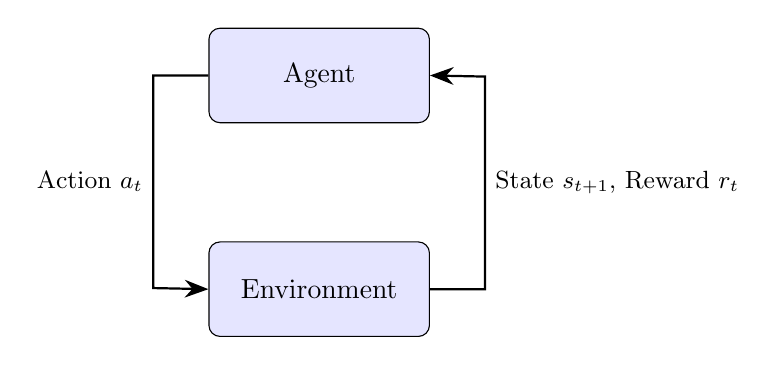
\begin{tikzpicture}[
      box/.style={rectangle, draw, minimum width=2.8cm, minimum height=1.2cm, text centered, rounded corners, fill=blue!10},
      arrow/.style={-{Stealth[length=3mm]}, thick},
      node distance=1.5cm and 1.5cm
    ]

    % Nodes
    \node[box] (agent) {Agent};
    \node[box, below=of agent] (env) {Environment};

    % Arrows
    \draw[arrow] (agent.west) -- ++(-0.7,0) -- ++(0,-1.35) node[left]{\small Action $a_t$} -- ++(0,-1.35) -- (env.west);
    \draw[arrow] (env.east) -- ++(0.7, 0) -- ++ (0,1.35) node[right] {\small State $s_{t+1}$, Reward $r_t$} -- ++ (0,1.35) -- (agent.east);

    \end{tikzpicture}
    \caption{Agent-environment interaction in reinforcement learning.}
    \label{fig:rl_loop}
\end{figure}

In RL, we are trying to create an agent, like a "brain," using a computer. This agent and environment interaction is often framed as a \textbf{Markov Decision Process (MDP)}. An MDP is a discrete sequence repeating as follows: 

\[ s_0, a_0, r_0, s_1, a_1, r_1, s_2, a_2, r_2, \dots \]

Where $s_i$ is the state, $a_i$ is the action taken and $r_i$ is a \textbf{reward signal}, which is a single number received after each action. It is representing whether the action had a good or bad outcome (more positive is better, more negative is worse). Conventionally, the reward is considered a signal from the environment to the agent. This sequence can either continue indefinitely or terminate, in which case it's called an \textbf{episode}.

Note that in the notation we are using here, each reward is associated with the timestamp of the preceding state and action. Other sources may instead align the reward with the resulting state and action, using a sequence like $s_0, a_0, r_1, s_1, ...$. This difference is not critical, but as a result, you may notice that some of the formulas presented here differ slightly from those found in other references. Additionally, while some sources use uppercase letters (e.g., capital R) to denote the reward, we have chosen to use lowercase r for consistency.

Ideally, the sequence in an MDP should follow the \textbf{Markov property}, meaning that \textit{each state is only dependent on its immediately previous state, not any earlier ones}. This ensures that the current state provides sufficient information to decide on the next action. For example, let's try to make a robot catch a ball:

\paragraph{Scenario 1:}

If the state information the robot receives only includes its own position $state = (position_x, position_y)$, then it's unclear what the next state will be. This is because the robot doesn't know the direction or speed at which the ball is moving. To deduce that information, the robot would have to look at multiple consecutive states. In this scenario, because determining the next state requires information from states before the immediately previous one (to figure out the ball's movement), the Markov property is not satisfied.

\paragraph{Scenario 2:}

If you include the velocity in the state information as well $state = (position_x, \\ position_y, velocity_x, velocity_y)$, then the state would follow the Markov property. With both position and velocity included, each state is only determined by the immediately previous one. This means there is sufficient information in the current state for the robot to potentially learn how one state transitions to the next, even if it doesn't understand things like gravity. Therefore, the state needs to contain enough relevant information from the environment for the Markov property to hold, ensuring that the current state is sufficient for deciding on the next action without needing a history of past states.

\bigskip

While many RL methods rely on this property, not all real-world situations satisfy it, and the MDP framework can be limited in dealing with varying time scales or tasks that require nuanced feedback beyond a single reward number. Despite these limitations, almost all of RL is built upon the foundation of MDPs.

Within an MDP, the ultimate goal of the agent is to figure out how to, for any given state, decide on an action that maximizes the total subsequent reward over time. To formalize this, two mathematical constructs are used:

\begin{itemize}[label={}]
    \item\textbf{Policy ($\pi$):} The strategy that takes a state as input and decides on an action as output $\pi:s \rightarrow a$. Technically, the policy usually represents the probability of picking a certain action given a state, allowing for randomness which is important for exploring different strategies. That's why in RL, the policy function is usually written as $\pi(a|s)$, which is the probability of picking a certain action, given—the '|' is a conditional—a certain state.
    \item\textbf{Return ($G_t$):} The total cumulative reward over time, starting from time step $t$ and ending at the last step $n$ which ends the episode (which could never happen). This is typically calculated as the sum of future rewards, progressively multiplied by a \textbf{discount factor gamma} $\gamma \in [0, 1]$. A lower gamma makes future rewards less significant, which can be useful if the future is hard to predict. If gamma is 1, it's an \textbf{undiscounted sum}, only suitable for terminating episodes to avoid infinite return. The goal is to \textbf{maximize the total reward over time}, not just the immediate reward.
\end{itemize}

\[ G_t = \sum_{k=0}^{n} \gamma^k r_{t+k+1} \]

Using this terminology, the goal is to find \textit{the policy ($\pi$) which maximizes return (G$_t$)}.

\section{The Maze Example}

We introduce a simple grid example, specifically a \textbf{maze}, to demonstrate key concepts in Reinforcement Learning (RL). The reason for using a grid, even though real-life problems are not this simple, is that it simplifies visualization and demonstration of concepts. Illustration is a lot easier when we're working with a simple example. 

\begin{center}
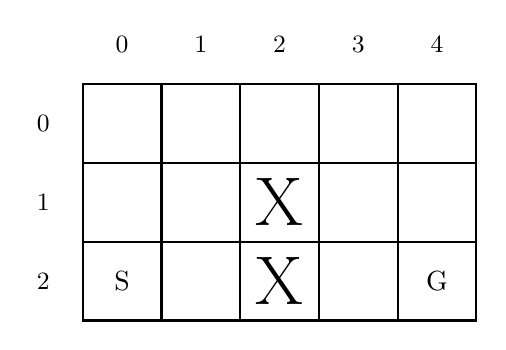
\begin{tikzpicture}
  % Draw the grid
  \foreach \x in {0,1,2,3,4} {
    \foreach \y in {0,1,2} {
      \draw[thick] (\x, \y) rectangle ++(1,-1);
    }
  }

  % Label start and goal
  \node at (0.5, -0.5) {S}; % (2,0)
  \node at (4.5, -0.5) {G}; % (2,4)

  % Draw walls as X
  \node at (2.5, -0.5) {\Huge X}; % (1,2)
  \node at (2.5, 0.5) {\Huge X}; % (2,2)

  % Index the columns
  \foreach \x in {0,1,2,3,4} {
    \node at (\x + 0.5, 2.5) {\small \x}; % column index above
  }

  % Index the lines
  \foreach \x in {0,1,2} {
      \pgfmathsetmacro{\label}{int(2 - \x)}
    \node at (-0.5, \x - 0.5) {\small \label}; % column index above
  }
\end{tikzpicture}
\end{center}

In this maze, the agent starts on a \textbf{starting cell \textit{(S)}} and must reach a \textbf{Target cell \textit{(G)}} by moving \textbf{up}, \textbf{down}, \textbf{left}, or \textbf{right}, and it \textbf{cannot move through walls}. There is a \textbf{maximum episode length of 20 steps}, meaning the episode \textbf{terminates} if the agent reaches the target or if 20 steps have passed without reaching it. To solve this task, the problem is framed as a Markov Decision Process (MDP):

\begin{itemize}[label={}]

    \item\textbf{State:} Each state is defined by two numbers $(x, y)$ representing the XY coordinates of the cell the agent is currently on.
    \item\textbf{Action:} Each action $a \in \{0, 1, 2, 3\}$ is a single number between zero and three, representing up, down, left, and right movement respectively.
    \item\textbf{Reward:} The reward $r$ after each action is 

\[ r =  \begin{cases}
            0 & \text{if the agent enters the target cell} \\
            -1 & \text{otherwise}
        \end{cases}
\]
    This reward structure incentivizes the agent to reach the target as fast as possible.

    \item\textbf{World Model:} As humans, we can see the whole maze, understand that states are coordinates, actions are directions, and how the reward system works. We understand, for instance, that moving right from (0,0) leads to (1,0) with a -1 reward, or hitting a wall keeps you in the same state. An agent that understands this is said to have a \textbf{world model}. Mathematically, this means having access to a function $P$ that predicts the next state and reward given a current state and action: $P:s,a \rightarrow s',r$, possibly accounting for randomness: $P(s',r|s,a)$.

\end{itemize}

Whether an RL agent has access to a world model makes a massive difference to how well it can learn to do tasks. This is why a lot of the current research in RL is concerned with how to develop better world models or make agents learn them on their own for complex tasks. Learning without a world model is referred to as \textbf{model-free reinforcement learning}. \textbf{Model-free methods}, which assume the agent doesn't understand what the state and action numbers mean or how rewards work, are not a very practical way of learning.

The inefficiency of model-free learning is illustrated with the tennis ball example. If an agent is trying to learn not to drop a tennis ball and lose points when it touches the table, without a world model (understanding of gravity, inertia, contact), it would just have to try letting go of the ball in numerous spots. It might take "300 trials" just to figure out that letting go above one half of the table makes you lose points, and then "another 300 trials" for the other half. This trial-and-error approach without basic environmental understanding is slow and inefficient. As humans, we rely on a world model, which is essential to understanding what's going to happen in everyday tasks like folding a t-shirt or walking. Having a world model allows the agent to imagine and simulate how things will turn out. This simulation can be used to train the agent with imagined experiences or to plan ahead while performing the task. Model-based reinforcement learning is considered a key subfield of future research that could help resolve issues like the sample inefficiency (we'll learn what this is in a moment) of current RL methods.

However, we choose to focuse on model-free methods. The agent cannot see the whole maze or understand what the state and action numbers represent or how rewards work; they are just meaningless random numbers. The agent's goal is to learn how to pick actions to maximize the rewards it receives.

\subsection{Policy Optimization}

Without any initial understanding, the agent starts by randomly picking actions. This means that, instead of using a policy with meaningful probabilities associated with each action — for example

\begin{figure}[H]
    \centering
    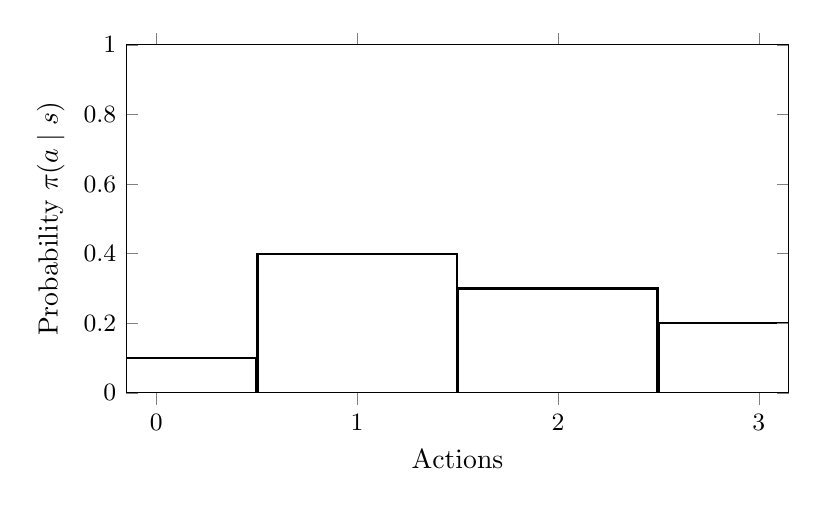
\begin{tikzpicture}
        \begin{axis}[
                ybar,
                bar width=72pt,
                ymin=0,
                ymax=1,
                ylabel={Probability $\pi(a \mid s)$},
                xlabel={Actions},
                symbolic x coords={0,1,2,3},
                xtick=data,
                enlarge x limits=0.05,
                axis on top,
%                nodes near coords,
                every node near coord/.append style={font=\small},
                major grid style={white},
                yticklabel style={font=\small},
                xticklabel style={font=\small},
                width=10cm,
                height=6cm,
            ]
            \addplot+[
                ybar,
                area legend,
                draw=black,
                thick,
                fill=white!50,
                bar shift=0pt
            ] coordinates {
                (0,0.1)
                (1,0.4)
                (2,0.3)
                (3,0.2)
            };
        \end{axis}
    \end{tikzpicture}
%    \caption{A policy distribution over actions with thick bars and clean background}
\end{figure}

It is effectively using a policy that looks like this:

\begin{figure}[H]
    \centering
    \begin{tikzpicture}
        \begin{axis}[
                ybar,
                bar width=72pt,
                ymin=0,
                ymax=1,
                ylabel={Probability $\pi(a \mid s)$},
                xlabel={Actions},
                symbolic x coords={0,1,2,3},
                xtick=data,
                enlarge x limits=0.05,
                axis on top,
%                nodes near coords,
                every node near coord/.append style={font=\small},
                major grid style={white},
                yticklabel style={font=\small},
                xticklabel style={font=\small},
                width=10cm,
                height=6cm,
            ]
            \addplot+[
                ybar,
                area legend,
                draw=black,
                thick,
                fill=white!50,
                bar shift=0pt
            ] coordinates {
                (0,0.25)
                (1,0.25)
                (2,0.25)
                (3,0.25)
            };
        \end{axis}
    \end{tikzpicture}
%    \caption{A policy distribution over actions with thick bars and clean background}
\end{figure}

For all these meaningless input numbers (action + state), the output numbers (the probabilities of selecting each action) are all the same. In other words, the policy is initially uniform and uninformative. The goal, of course, is to improve this policy over time. But initially, since actions are chosen almost entirely at random, the agent performs poorly—typically receiving a total reward of -20, as each episode is limited to 20 steps. However, what the agent does achieve is recording all of its experiences during each episode, which can later be used for learning.

This process of trying actions and collecting sequences of states, actions, and rewards (known as \textbf{trajectories} or \textbf{sample trajectories}) is called \textbf{sampling}. These samples are recorded in tables, where we also calculate the return for each step using a discount factor of $\gamma = 0.8$:

% Creating a table to record an episode
\begin{table}[h!]
    \centering
%    \caption{Example Episode in the Maze}
    \begin{tabular}{|c|c|c|c|c|}
        \toprule
        \textbf{State} & \textbf{Action} & \textbf{Next State} & \textbf{Reward} & \textbf{Return} \\
        \midrule
        (2,0) & 3 (right) & (2,1) & -1 & -4.94 \\
        (2,1) & 0 (up) & (1,1) & -1 & -4.93 \\
        $\vdots$ & $\vdots$ & $\vdots$ & $\vdots$ & $\vdots$ \\
        (1,1) & 1 (down) & (2,1) & -1 & -1.8 \\
        (2,1) & 0 (up) & (1,1) & -1 & -1 \\
        \bottomrule
    \end{tabular}
\end{table}

Note that the final reward is $-1$, which means that the agent made no progress in that episode. Naturally, this results in all rewards and returns being negative—except in rare, lucky episodes where the agent succeeds. In such cases, the recorded table would look more like this:

\begin{table}[h!]
    \centering
    \begin{tabular}{|c|c|c|c|c|}
        \toprule
        \textbf{State} & \textbf{Action} & \textbf{Next State} & \textbf{Reward} & \textbf{Return} \\
        \midrule
        (2,0) & 3 (right) & (2,1) & -1 & -4.33 \\
        (2,1) & 0 (up) & (1,1) & -1 & -4.16 \\
        $\vdots$ & $\vdots$ & $\vdots$ & $\vdots$ & $\vdots$ \\
        (1,3) & 1 (down) & (2,3) & -1 & -1 \\
        (2,3) & 3 (right) & (4,2) & 0 & 0 \\
        \bottomrule
    \end{tabular}
\end{table}

The next step is to use these experiences to improve the policy. We need a way to evaluate the actions we took so that we can adjust the policy in favor of the better ones. To do this, we use a concept called the \textbf{action-value function}, denoted by \textbf{$Q$}. The \textbf{$Q-value$} of a given state $s$ and action $a$, written as $Q^{\pi}(s,a)$, is an estimate of the expected return starting from state $s$, taking action $a$, and then following the policy $\pi$. Expressed mathematically, we aim to approximate 

\[ \mathbb{E}_\pi[G_t \mid s_t = s, a_t = a] \]

Of course, we have to construct this function ourselves. To do so, we can use the trajectories we collected and compute the average of the return values for each state-action pair. We can imagine that, initially, the Q-function assigns a value of 0 to every possible state-action input, as illustrated in the following table:

\begin{table}[H]
    \centering
%    \caption{Initial Q-Function for State-Action Pairs}
    \begin{tabular}{|c|c|c|c|c|}
        \toprule
        \textbf{State} & \textbf{$Q(s, 0)$ (Up)} & \textbf{$Q(s,1)$ (Down)} & \textbf{$Q(s,2)$ (Left)} & \textbf{$Q(s,3)$ (Right)} \\
        \midrule
        (0,2) & 0 & 0 & 0 & 0 \\
        (1,2) & 0 & 0 & 0 & 0 \\
        \vdots & \vdots & \vdots & \vdots & \vdots \\
        (3,2) & 0 & 0 & 0 & 0 \\
        (4,2) & 0 & 0 & 0 & 0 \\
        \bottomrule
    \end{tabular}
\end{table}

For each state-action pair \( (s, a) \) in a trajectory, we will move the Q-value towards the pre-computed return \( G \) by a small amount. The is done using the formula:

\[ Q(s, a) \leftarrow Q(s, a) + \alpha \left[ G - Q(s, a) \right] \]

where \( \alpha \in (0, 1] \) (e.g., \( \alpha = 0.1 \)) is the \textbf{learning rate}, controlling the step size toward the target return. This update adjusts the Q-value based on the difference between the observed return and the current estimate, ensuring gradual convergence. When the same state-action pair is revisited in subsequent trajectories, the updated Q-value serves as the new baseline, effectively computing a running average of returns. This process increases Q-values for actions that yield higher returns (e.g., moving toward the goal) while decreasing those for less effective actions (e.g., hitting walls).

To illustrate, consider the state-action pair \( ((1,2), 0) \) (action up from state (1,2)). We demonstrate two updates using pre-computed returns:

\begin{enumerate}[label=\roman*.]

    \item \textbf{Trajectory 1}: In the successful trajectory (Table 2), the pair \( ((2,1), 0) \) has a return \( G = -4.16 \). Assuming an initial \( Q((2,1), 0) = 0 \) and \( \alpha = 0.1 \), the update is:

    \[ Q((1,2), 0) \leftarrow 0 + 0.1 \cdot (-4.16 - 0) = -0.416 \]

    \item \textbf{Trajectory 2}: In the unsuccessful trajectory (Table 1), the pair \( ((2,1), 0) \) with a return \( G = -4.93 \). Using the updated \( Q((2,1), 0) = -0.416 \) the update is:

    \[ Q((1,2), 0) \leftarrow -0.416 + 0.1 \cdot (-4.93 - (-0.416)) = -0.416 + 0.1 \cdot (-4.514) = -0.4514 \]

\end{enumerate}

These updates demonstrate how \( Q((2,1), 0) \) evolves toward the average return, reflecting the action’s limited effectiveness (as it hits a wall at (2,2)). Over multiple trajectories, Q-values for effective actions converge to higher values, improving the accuracy of its evaluation.

\bigskip

The \( Q \)-function serves as the foundation for the agent’s decision-making process. It enables the evaluation of state-action pairs, defines the policy through action selection, and facilitates iterative policy improvement. Below, we detail the primary roles of the \( Q \)-function in shaping the agent’s policy within the context of the maze example.

\begin{enumerate}[label={}, leftmargin=0pt]
    
    \item \textbf{Greedy Policy Definition}

    The agent \textbf{exploits} by selecting the action with the highest \( Q \)-value in each state, i.e., \( a^* = \arg\max_a Q(s, a) \). This greedy approach, termed \textbf{exploitation}, leverages the \( Q \)-function to maximize expected rewards based on current estimates.    

    \item \textbf{Balancing Exploration and Exploitation}

    Exclusive reliance on greedy selection risks overlooking better actions due to limited \textbf{exploration}, particularly when \( Q \)-values are based on few samples. To address this, the agent employs an \textbf{epsilon-greedy strategy}:

    \begin{itemize}[label={}]
        \item With probability \( 1 - \epsilon \), the agent exploits by selecting the action with the highest \( Q \)-value for the current state.
        \item With probability \( \epsilon \), the agent explores by choosing a random action, ensuring all actions are sampled over time.
    \end{itemize}

    Thus, 

\[ \pi(a|s) =    \begin{cases}
                    1 - \epsilon + \epsilon / |A| & \text{for the greedy action $a = \arg\max_a Q(s, a)$} \\
                    \epsilon / |A| & \text{for other actions $a \neq \arg\max_a Q(s, a)$}
                \end{cases}
\]

    for each $(action,state)$ pair. Where $A$ is the set of possible actions. For instance, \( |A| = 4 \) in the maze. For example, in state (2,1), if \( Q((2,1), 3) = -0.19 \) (right) exceeds \( Q((2,1), 0) = -0.4744 \) (up), and \( \epsilon = 0.2 \), the policy becomes \( \pi(3|(2,1)) = 0.8 + 0.2/4 = 0.85 \), with \( \pi(a|(2,1)) = 0.05 \) for others. Therefore, the policy would initially be uniform, with \( Q(s, a) = 0 \) (i.e., \( \pi(a|s) = 0.25 \)). As more iterations adjust Q-values, the policy shifts to favor actions with higher Q-values, aligning with more rewarding paths.
        
    \item \textbf{Epsilon Decay}: 

    To balance exploration and exploitation, \( \epsilon \) is initialized at a high value (e.g., \( \epsilon = 0.5 \)) to encourage exploration when \( Q \)-values are unreliable. As the \( Q \)-function is refined, \( \epsilon \) is gradually reduced (e.g., to \( \epsilon = 0.1 \)), allowing the agent to increasingly favor exploitation of learned values. This transforms the policy from a uniform distribution to one concentrated on the optimal action.

\end{enumerate}

This interplay of evaluation and policy improvement exemplifies \textbf{generalized policy iteration}. The agent evaluates its policy by updating \( Q \)-values, as shown in prior examples, and improves its policy by selecting actions based on these values, refined by this method, which is called the \textbf{Monte Carlo Method}.

% Summarizing the Python code
\subsection{Code Implementation}

In the Python implementation. The agent learns by generating a 1000 episodes with an epsilon-greedy policy (\(\epsilon\) from 0.5 to 0.1, decay 0.995). At the end of it's training, the program's output was the following:

% Q-Table Matrix
\subsubsection{Q-Table Matrix}

The Q-table shows Q-values for actions: Up (0), Down (1), Left (2), Right (3). Special states are marked: Start (S), Goal (G), Wall (X).

\begin{table}[h]
    \centering
    \resizebox{\textwidth}{!}{
    \begin{tabular}{|c|*{5}{c|}}
        \toprule
        \textbf{Row} & \multicolumn{5}{c|}{\textbf{Column (y)}} \\
        \cmidrule{2-6}
        \textbf{(x)} & 0 & 1 & 2 & 3 & 4 \\
        \midrule
        2 & [S] & [-4.34, -3.92, -4.40, -4.35] & [X] & [-1.96, -1.17, -1.58, 0.00] & [G] \\
        1 & [-4.30, -3.77, -4.11, -3.98] & [-4.17, -3.71, -4.23, -4.02] & [X] & [-1.23, -2.49, -2.16, -1.07] & [0.00, -1.80, -1.38, -0.95] \\
        0 & [-4.21, -4.19, -4.01, -3.44] & [-3.87, -3.62, -3.82, -3.03] & [-3.02, -3.12, -3.52, -2.52] & [-1.90, -2.77, -3.05, -2.33] & [-1.47, -1.98, -2.51, -1.91] \\
        \bottomrule
    \end{tabular}
    }
    \caption{Q-Table Matrix (Q-values: Up, Down, Left, Right)}
\end{table}

\begin{figure}[H]
    \centering
    \includegraphics[width=0.8\textwidth]{total_rewards.png}
    \caption{Total undiscounted reward per episode over 1000 episodes.}
\end{figure}

\begin{figure}[H]
    \centering
    \includegraphics[width=0.8\textwidth]{policy_maze.png}
    \caption{Policy visualization: arrows indicate the optimal action (highest Q-value) for each state in the 5$\times$3 maze.}
\end{figure}

\section{Temporal Difference}
\label{sec:td_learning}

% Introducing Temporal Difference Learning
Among the many limitations of the Monte Carlo method is the need to wait for an entire episode to end to calculate returns, that makes it hard to know which action during our process was optimal and which wasn't within a long sequence of actions. This is a well-known issue in RL, called the \textbf{Credit Assignment Problem}.

Without having access to a world-model, a common solution is a concept called \textbf{Temporal Difference (TD)}, which is a blending between the sample-based learning of Monte Carlo methods and the \textbf{bootstrapping} approach of \textbf{dynamic programming}. It offers a solution to these issues by breaking down evaluation to an action-by-action basis. Instead of waiting for the sum of all subsequent rewards (the return), TD methods learn by upgrading their $Q-value$ for a given state-action pair $(s_t,a_t)$, using the $Q-value$ of the state $s_{t+1}$ in the time step after it and just the one immediate reward $r_t$. 

In RL, the goal is to maximize the expected return, defined as the cumulative discounted reward starting from time step \( t \):

\[
G_t = \sum_{k=0}^\infty \gamma^k r_{t+k+1}
\]

where \( r_{t+k+1} \) is the reward received after taking action \( a_{t+k} \) in state \( s_{t+k} \), and \( \gamma \in [0,1] \) is the discount factor. A key insight is that the return can be expressed recursively:

\[
G_t = r_t + \gamma G_{t+1}
\]

This recursive relationship shows that the return at time \( t \) is the immediate reward \( r_t \) plus the discounted return from the next time step \( G_{t+1} \). Using the recursive return, the TD learning approach estimates \( Q(s_t, a_t) \) by moving it toward the immediate reward plus the discounted value of the next state-action pair:

\[
Q(s_t, a_t) \leftarrow Q(s_t, a_t) + \alpha \left[ r_t + \gamma Q(s_{t+1}, a_{t+1}) - Q(s_t, a_t) \right]
\]

Here, \( \alpha \in (0,1] \) is the learning rate, and the term \( r_t + \gamma Q(s_{t+1}, a_{t+1}) \) serves as a target for the update. The difference \( r_t + \gamma Q(s_{t+1}, a_{t+1}) - Q(s_t, a_t) \), known as the \textbf{TD error}, measures the discrepancy between the current estimate and the new evidence from the sample trajectory. This update is model-free, as it relies solely on observed transitions without requiring a world model.

\subsection{TD Learning Methods}

The TD update rule varies across methods based on how the next state-action pair’s value is estimated. We discuss three prominent TD methods: Q-learning, SARSA, and Expected SARSA, and their application to the maze example.

\begin{enumerate}[label={}, leftmargin=0pt]

    \item\textbf{Q-learning} is an off-policy TD method that updates Q-values using the maximum value of the next state’s actions, regardless of the policy followed:

    \[
    Q(s_t, a_t) \leftarrow Q(s_t, a_t) + \alpha \left[ r_t + \gamma \max_{a'} Q(s_{t+1}, a') - Q(s_t, a_t) \right]
    \]

\item\textbf{SARSA} (State-Action-Reward-State-Action) is an on-policy TD method that uses the actual action taken in the next state, following the current policy \( \pi \):

    \[
    Q(s_t, a_t) \leftarrow Q(s_t, a_t) + \alpha \left[ r_t + \gamma Q(s_{t+1}, a_{t+1}) - Q(s_t, a_t) \right]
    \]

    \item\textbf{Expected SARSA} improves on SARSA by using the expected value of the next state’s actions, weighted by the policy’s probabilities:

    \[
    Q(s_t, a_t) \leftarrow Q(s_t, a_t) + \alpha \left[ r_t + \gamma \sum_{a'} \pi(a' \mid s_{t+1}) Q(s_{t+1}, a') - Q(s_t, a_t) \right]
    \]

\end{enumerate}

Algorithms are classified as on-policy or off-policy based on the relationship between the policy used to select actions (the behavior policy) and the policy being evaluated or improved (the target policy). An \textbf{on-policy} algorithm learns the value of the policy it is currently following. The behavior policy and the target policy are the same. On the other hand, \textbf{off-policy} algorithms learn the value of a different policy (typically the optimal policy) than the one used to select actions.

\subsection{Implementation}

In this section we implemented the Q-learning algorithm in the same maze environment as the previous section. We did this because we want to compare Monte Carlo with Q-learnign to see which is more sample efficient. \textbf{Sample efficiency} refers to the number of samples (either the number of episodes or the number of time steps) that it takes for an agent to get good at a task. If one method requires fewer samples to achieve good performance compared to another, it is considered more sample efficient.

Looking at the results of both algorithms, the result isn't too different. Q-learning is only doing slightly better.

\begin{figure}[H]
    \centering
    \begin{subfigure}[t]{0.45\textwidth}
        \centering
        \includegraphics[width=\linewidth]{moving_avg_reward.png}
        \caption{Monte Carlo}
        \label{fig:image1}
    \end{subfigure}
    \hfill
    \begin{subfigure}[t]{0.45\textwidth}
        \centering
        \includegraphics[width=\linewidth]{Q-moving_avg_reward.png}
        \caption{Q-learning}
        \label{fig:image2}
    \end{subfigure}
    \caption{Comparison Monte Carlo - Q-Learning}
    \label{fig:combined}
\end{figure}

However, the moment we switch to a bigger maze, then the difference is staggering:

\begin{figure}[H]
    \centering
    \begin{subfigure}[t]{0.45\textwidth}
        \centering
        \includegraphics[width=\linewidth]{Newmoving_avg_reward.png}
        \caption{Monte Carlo}
    \end{subfigure}
    \hfill
    \begin{subfigure}[t]{0.45\textwidth}
        \centering
        \includegraphics[width=\linewidth]{NewQ-moving_avg_reward.png}
        \caption{Q-learning}
    \end{subfigure}
    \caption{Comparison is the thief of joy}
\end{figure}

Monte Carlo isn't able to reach the target square even once. The benefits of a more efficient algorithm really starts to show in a more complex environment.

\chapter{Advanced Concepts in Reinforcement Learning}

\section{Value Functions and Bellman Equations}
\label{sec:value_functions}

% Introducing the concept of value functions
In reinforcement learning (RL), a critical component for decision-making is the ability to evaluate the long-term desirability of states or state-action pairs. This is achieved through \emph{value functions}, which estimate the expected cumulative reward an agent can achieve starting from a given state or state-action pair, following a specific policy. Value functions provide a quantitative measure of how ``good'' a state or action is in terms of future rewards, guiding the agent toward optimal decisions. In this section, we explore two primary types of value functions---the state-value function and the action-value function---and introduce the Bellman equations, which are foundational to RL algorithms.

\subsection{State-Value and Action-Value Functions}

The \emph{state-value function}, denoted \( V^\pi(s) \), represents the expected return (cumulative discounted reward) when starting in state \( s \) and following policy \( \pi \) thereafter. Mathematically, it is defined as:

\[
V^\pi(s) = \mathbb{E}_\pi \left[ G_t \mid S_t = s \right] = \mathbb{E}_\pi \left[ \sum_{k=0}^\infty \gamma^k r_{t+k+1} \mid S_t = s \right]
\]

where \( G_t \) is the return at time \( t \), \( \gamma \in [0,1] \) is the discount factor, and the expectation is taken over the trajectories generated by policy \( \pi \). The state-value function quantifies the long-term value of being in a particular state, assuming the agent follows the policy.

The state-value function is related to the Q-function by averaging over the policy:

\[
V^\pi(s) = \sum_{a} \pi(a|s) Q^\pi(s, a)
\]

This means the value of a state is the average of the Q-values for all possible actions, weighted by the policy’s preference for each action.


The \emph{action-value function}, denoted \( Q^\pi(s, a) \), was introduced in Section~\ref{sec:maze_example} and represents the expected return when starting in state \( s \), taking action \( a \), and then following policy \( \pi \). It is defined as:

\[
Q^\pi(s, a) = \mathbb{E}_\pi \left[ G_t \mid S_t = s, A_t = a \right] = \mathbb{E}_\pi \left[ \sum_{k=0}^\infty \gamma^k r_{t+k+1} \mid S_t = s, A_t = a \right]
\]

\textbf{Optimal State-Value Function (\( V^* \))}: The optimal state-value function represents the maximum total reward an agent can achieve from a state by following the best possible policy. It indicates the highest value a state can have.

\textbf{Optimal Action-Value Function (\( Q^* \))}: The optimal action-value function represents the maximum total reward an agent can achieve by taking a specific action in a state and then following the best possible policy. It evaluates the best possible action in each state.

\subsection{Bellman Equations}

The Bellman equations provide a recursive formulation of value functions, breaking down the expected return into the immediate reward and the value of the next state. This recursive structure is crucial for both evaluating and improving policies in RL.

For the state-value function, the Bellman equation is:

\[
V^\pi(s) = \mathbb{E}_\pi \left[ r_{t+1} + \gamma V^\pi(s_{t+1}) \mid S_t = s \right]
\]

This equation states that the value of state \( s \) under policy \( \pi \) is the expected immediate reward \( r_{t+1} \) plus the discounted value of the next state \( s_{t+1} \), averaged over all possible actions and next states according to the policy and environment dynamics.

For the action-value function, the Bellman equation is:

\[
Q^\pi(s, a) = \mathbb{E}_\pi \left[ r_{t+1} + \gamma \sum_{a' \in A} \pi(a' \mid s_{t+1}) Q^\pi(s_{t+1}, a') \mid S_t = s, A_t = a \right]
\]

This expresses the value of taking action \( a \) in state \( s \) as the expected immediate reward plus the discounted expected value of the next state-action pairs, weighted by the policy's action probabilities.

\subsection{Policy Gradient Methods}

Policy gradient methods are a class of RL algorithms that directly improve the policy to maximize total rewards. Unlike Monte Carlo or Q-Learning, which estimate values to select actions, these methods adjust the policy itself. Policy gradient methods are vital for tasks requiring complex or continuous policies, such as robotic control or games with large action spaces. They enable agents to learn sophisticated strategies directly. 

These methods emerged from the need to optimize policies directly, rather than relying on value estimates, allowing for more flexible and complex policy learning. It handles complex and continuous action spaces effectively, suitable for tasks with large or infinite action sets and offers flexibility in designing policies. It is however less stable than value-based methods. and requires more samples to learn effectively. In addition, sensitive to learning rate and other parameters.
\begin{thebibliography}{9}
    \bibitem{rlhf2025}
    Reinforcement Learning in 2025: Benefits \& Applications,
    \url{https://research.aimultiple.com/reinforcement-learning/}.

    \bibitem{deepmindfusion}
    DeepMind, Advancing Nuclear Fusion with Machine Learning,
    \url{https://www.deepmind.com/blog/advancing-nuclear-fusion-with-machine-learning}.

    \bibitem{marktechpost2024}
    MarkTechPost, Discover How Reinforcement Learning and Language Models Are Revolutionizing Protein Sequence Design,
    \url{https://www.marktechpost.com/2024/07/08/discover-how-reinforcement-learning-and-language-models-are-revolutionizing-protein-sequence-design/}.

    \bibitem{kommey2024}
    Kommey, B., et al., A Reinforcement Learning Review: Past Acts, Present Facts and Future Prospects,
    \url{https://www.researchgate.net/publication/378250885_Reinforcement_Learning_Review_Past_Acts_Present_Facts_and_Future_Prospects}.

    \bibitem{aiindex2025}
    Stanford HAI, AI Index 2025 Report,
    \url{https://hai.stanford.edu/ai-index/2025-ai-index-report}.

    \bibitem{mdpi2023}
    A Systematic Study on Reinforcement Learning Based Applications,
    \url{https://www.mdpi.com/1996-1073/16/3/1512}.

    \bibitem{xrl2024}
    Explainable Reinforcement Learning: A Survey and Comparative Review,
    \url{https://dl.acm.org/doi/10.1145/3616864}.

    \bibitem{rlalgorithms2023}
    Reinforcement Learning Algorithms: A Brief Survey,
    \url{https://www.sciencedirect.com/science/article/abs/pii/S0957417423009971}.

    \bibitem{wiki2025}
    Wikipedia, Age of Artificial Intelligence,
    \url{https://en.wikipedia.org/wiki/Age_of_artificial_intelligence}.
\end{thebibliography}

\end{document}  % End of the document
